%%%%%%%%%%%%%%%%%%%%%%%%%%%%%%%%%%%%%%%%%
% Stylish Article
% LaTeX Template
% Version 2.2 (2020-10-22)
%
% This template has been downloaded from:
% http://www.LaTeXTemplates.com
%
% Original author:
% Mathias Legrand (legrand.mathias@gmail.com) 
% With extensive modifications by:
% Vel (vel@latextemplates.com)
%
% License:
% CC BY-NC-SA 3.0 (http://creativecommons.org/licenses/by-nc-sa/3.0/)
%
%%%%%%%%%%%%%%%%%%%%%%%%%%%%%%%%%%%%%%%%%

%----------------------------------------------------------------------------------------
%	PACKAGES AND OTHER DOCUMENT CONFIGURATIONS
%----------------------------------------------------------------------------------------

\documentclass[fleqn,10pt]{SelfArx} % Document font size and equations flushed left

\usepackage[spanish, mexico]{babel} % Specify a different language here - english by default
%\usepackage[english]{babel}
\usepackage{lipsum} % Required to insert dummy text. To be removed otherwise


\usepackage{listings}
\usepackage{xcolor}

\definecolor{codegreen}{rgb}{0,0.6,0}
\definecolor{codegray}{rgb}{0.5,0.5,0.5}
\definecolor{codepurple}{rgb}{0.58,0,0.82}
\definecolor{backcolour}{rgb}{0.95,0.95,0.92}

\lstdefinestyle{mystyle}{
    backgroundcolor=\color{backcolour},   
    commentstyle=\color{codegreen},
    keywordstyle=\color{magenta},
    numberstyle=\tiny\color{codegray},
    stringstyle=\color{codepurple},
    basicstyle=\ttfamily\footnotesize,
    breakatwhitespace=false,         
    breaklines=true,                 
    captionpos=b,                    
    keepspaces=true,                 
    numbers=left,                    
    numbersep=5pt,                  
    showspaces=false,                
    showstringspaces=false,
    showtabs=false,                  
    tabsize=2
}

\lstset{style=mystyle}

%----------------------------------------------------------------------------------------
%	COLUMNS
%----------------------------------------------------------------------------------------

\setlength{\columnsep}{0.55cm} % Distance between the two columns of text
\setlength{\fboxrule}{0.75pt} % Width of the border around the abstract

%----------------------------------------------------------------------------------------
%	COLORS
%----------------------------------------------------------------------------------------

\definecolor{color1}{RGB}{0,0,90} % Color of the article title and sections
\definecolor{color2}{RGB}{0,20,20} % Color of the boxes behind the abstract and headings

%----------------------------------------------------------------------------------------
%	HYPERLINKS
%----------------------------------------------------------------------------------------

\usepackage{hyperref} % Required for hyperlinks

\hypersetup{
	hidelinks,
	colorlinks,
	breaklinks=true,
	urlcolor=color2,
	citecolor=color1,
	linkcolor=color1,
	bookmarksopen=false,
	pdftitle={Title},
	pdfauthor={Author},
}

%----------------------------------------------------------------------------------------
%	ARTICLE INFORMATION
%----------------------------------------------------------------------------------------

%\JournalInfo{Journal, Vol. XXI, No. 1, 1-5, 2013} % Journal information
\JournalInfo{Semestre, 2020-1}
\Archive{Herramientas Computacionales} % Additional notes (e.g. copyright, DOI, review/research article)

\PaperTitle{Crecimiento de Poblaciones} % Article title

\Authors{Pedro Porras Flores\textsuperscript{1}*, Abraham Arellano Sánchez\textsuperscript{2}, María González Ramírez\textsuperscript{2}} % Authors
\affiliation{\textsuperscript{1}\textit{Departamento de Matemáticas y Mecánica, IMASS, UNAM}} % Author affiliation
\affiliation{\textsuperscript{2}\textit{Escuela Nacional de Ciencias de la Tierra, UNAM}} % Author affiliation
\affiliation{*\textbf{GitHub}: } % Corresponding author

\Keywords{Palabra clave 1, palabra clave 2, palabra clave 3, palabra clave 4.} % Keywords - if you don't want any simply remove all the text between the curly brackets
\newcommand{\keywordname}{Palabras clave} % Defines the keywords heading name

%----------------------------------------------------------------------------------------
%	ABSTRACT
%----------------------------------------------------------------------------------------

\Abstract{El resumen es un breve párrafo que generalmente no excede las 350 palabras, el cual contiene dos oraciones cortas de introducción sobre el tema del artículo y la razón de su publicación. A continuación se presentan los objetivos y alcances del artículo en pasado simple; es importante incluir las técnicas experimentales y de caracterización utilizadas. La siguiente sección incluye los resultados e información más relevante, incluyendo las unidades adecuadas (es válido, por ejemplo, expresar una velocidad como m/s o m s$^{-1}$). Las conclusiones resumen la información presentada previamente y se hace mención a la contribución científica e implicaciones potenciales de los descubrimientos. Es importante mencionar que el resumen es la última sección del artículo que debe ser redactada.}

%----------------------------------------------------------------------------------------

\begin{document}

\maketitle % Output the title and abstract box

\tableofcontents % Output the contents section

\thispagestyle{empty} % Removes page numbering from the first page

%----------------------------------------------------------------------------------------
%	ARTICLE CONTENTS
%----------------------------------------------------------------------------------------

\section*{Preámbulo}

Esto es un preámbulo 
%\subsection*{subsección 1}
La ecuación más hermosas del universo es: $e^{i \pi}  + 1 = 0$ \\ $\Omega$, $\hbar$

Este trabajo se basa en \cite{murray2007mathematical}
%\subsubsection*{subsubsección 1.1}
%\subsection*{subsección 2}
%\subsection*{subsección 3}
%\subsection*{subsección 4}

\section*{Introducción} % The \section*{} command stops section numbering

\addcontentsline{toc}{section}{Introducción} % Adds this section to the table of contents

La introducción es la sección donde se presenta el problema científico a resolver y se describe el contexto a evaluar durante el trabajo. Es importante partir de lo general a lo particular y no divagar, además de solo incluir información relevante y redactar objetivamente, sin utilizar palabras rebuscadas o complejas a menos que se utilice un concepto técnico.

En esta sección se deben describir los principios teóricos y trabajos previos que fundamenten los experimentos presentados a continuación. La información deberá ser obtenida de artículos científicos publicados en revistas indexadas; es posible citar libros y otras fuentes primarias, sin embargo, mayormente es necesario hacer referencia a artículos. Aquí deben de colocarse ecuaciones que pudiesen en ser de utilidad para explicar los principios químicos. En los laboratorios impartidos a los alumnos de INCQ, generalmente se les solicita como mínimo 4 referencias, sin embargo, se invita a utilizar todas las fuentes confiables que sean de utilidad.

A continuación, se mostrará cómo redactar ecuaciones, hacer referencias a estas en el texto y citar fuentes en esta plantilla. Por ejemplo, describamos la ecuación general de segundo grado:

\begin{equation}
    \label{eq:eg2}
    ax^2 + bx + c = 0
\end{equation}

La integral de, $\displaystyle \int_{0}^{2} x^2 \, dx$ es

La derivada $\dfrac{d}{dx} \left( \dfrac{1}{x} \right)$
La derivada $\displaystyle \sum_{k = 1}^{\infty} \left( \dfrac{1}{k} \right)$

\noindent donde $a$, $b$ y $c$ son los coeficientes de la ecuación (\ref{eq:eg2}). Para encontrar el valor de $x$, es necesario aplicar la siguiente solución:

\begin{equation}
    \label{eq:solucion}
    x = \displaystyle\frac{-b \pm \sqrt{b^2-4ac}}{2a}
\end{equation}

En un trabajo formal es necesario hacer referencia a todas las ecuaciones, figuras y tablas que se presenten; para lograr esto, será necesario agregar una etiqueta a cada elemento. El código necesario para obtener la ecuación \eqref{eq:eg2} es el siguiente:

\begin{verbatim}
    \begin{equation}
        \label{eq:eg2}
        ax^2 + bx + c = 0
    \end{equation}
\end{verbatim}

\noindent Cualquier información contenida en el ambiente \texttt{equation} resultará en un tipo de letra matemático, lo cual a su vez es posible ya que se han cargado paquetes específicos en el preámbulo. Para lograr la referencia en el texto, es necesario redactar el código \verb|\eqref{eq:eg2}|. Ahora revisemos cómo introducir la ecuación \eqref{eq:solucion} en el código de \LaTeX:

\begin{verbatim}
    \begin{equation}
        \label{eq:solucion}
        x = \displaystyle\frac{-b 
        \pm \sqrt{b^2-4ac}}{2a}
    \end{equation}
\end{verbatim}

\noindent Es importante mencionar que el código se escribe de manera continua, sin embargo, para mostrarse en este ejemplo fue separado en dos líneas.

En este conjunto de archivos resalta la presencia de aquel con nombre \texttt{sample.bib}. Este contiene la información necesaria para poder citar los artículos de interés; observemos por ejemplo el siguiente caso:

\begin{verbatim}
    @article{Ali2015,
        author = {Ali, Mohamed Kamal 
            Ahmed and Xianjun, Hou},
        doi = {10.1515/ntrev-2015-0031},
        journal = {Nanotechnology 
            Reviews},
        number = {4},
        pages = {347--358},
        title = {Simplified article
            title},
        volume = {4},
        year = {2015
    }
\end{verbatim}

Esta información puede descargarse en archivos \texttt{.bib} en la misma página donde se obtiene el artículo citado, sin embargo, puede generarse automáticamente utilizando Mendeley, entre otros gestores bibliográficos. Para hacer referencia en el texto a la cita anterior, será necesario usar el comando \verb|\cite{Ali2015}|, lo cual resultará en \cite{Ali2015}.%; el autor de esta plantilla ha desarrollado e incluido en el preámbulo el comando \verb|\cite{}|, lo cual resulta en resaltar en \textbf{negritas} la cita obtenida previamente, generando  \cite{Ali2015} a partir del código \verb|\cite{Ali2015}|, evitando redactar \verb|\textbf{\cite{Ali2015}}|. Además, si en las entradas bibliográficas (ejemplo anterior) se agrega el DOI de la fuente, en la sección de referencias se generará un hipervínculo en la entrada correspondiente dirigiendo al lector al URL de donde se obtuvo esta; revise por ejemplo $Francis2014$.

El último párrafo de la introducción describe explícita y detalladamente los objetivos del presente trabajo; es necesario también mencionar cuál o cuales son las diferencias que se han evaluado aquí en comparación con trabajos previos.

%\lipsum[1-3] % Dummy text
% and some mathematics $\cos\pi=-1$ and $\alpha$ in the text\footnote{And some mathematics $\cos\pi=-1$ and $\alpha$ in the text.}.

%------------------------------------------------

%%%%%%%%%%%%%%%%%%%%%%%%%%%%%%%%%%%%%%%%%%%%%%%%%
\section{Metodología} % NOMBRE DE LA SECCIÓN
%\label{sec:metodologia} % ETIQUETA
%%%%%%%%%%%%%%%%%%%%%%%%%%%%%%%%%%%%%%%%%%%%%%%%%

%------------------------------------------------
\subsection{Materiales y sustancias}
%\label{subsec:materiales-sustancias}
%------------------------------------------------

En esta subsección será necesario describir todos los reactivos utilizados, donde se deberá incluir el nombre del reactivo tal como aparece en la etiqueta y marca; se alienta al redactor a ser lo más explícito posible en la descripción de las sustancias. También, se deberán mencionar aquellos materiales, software y equipos de caracterización que fuesen utilizados. Es importante mencionar que los materiales de vidrio comunes (matraces, vasos, vidrios de reloj, etc.) no es necesario mencionarlos en esta sección ni redactar su marca u origen.


\begin{lstlisting}
import numpy as np
    
def incmatrix(genl1,genl2):
    m = len(genl1)
    n = len(genl2)
    M = None #to become the incidence matrix
    VT = np.zeros((n*m,1), int)  #dummy variable
    
    #compute the bitwise xor matrix
    M1 = bitxormatrix(genl1)
    M2 = np.triu(bitxormatrix(genl2),1) 

    for i in range(m-1):
        for j in range(i+1, m):
            [r,c] = np.where(M2 == M1[i,j])
            for k in range(len(r)):
                VT[(i)*n + r[k]] = 1;
                VT[(i)*n + c[k]] = 1;
                VT[(j)*n + r[k]] = 1;
                VT[(j)*n + c[k]] = 1;
                
                if M is None:
                    M = np.copy(VT)
                else:
                    M = np.concatenate((M, VT), 1)
                
                VT = np.zeros((n*m,1), int)
    
    return M
\end{lstlisting}
%\begin{figure*}[ht]\centering % Using \begin{figure*} makes the figure take up the entire width of the page
%	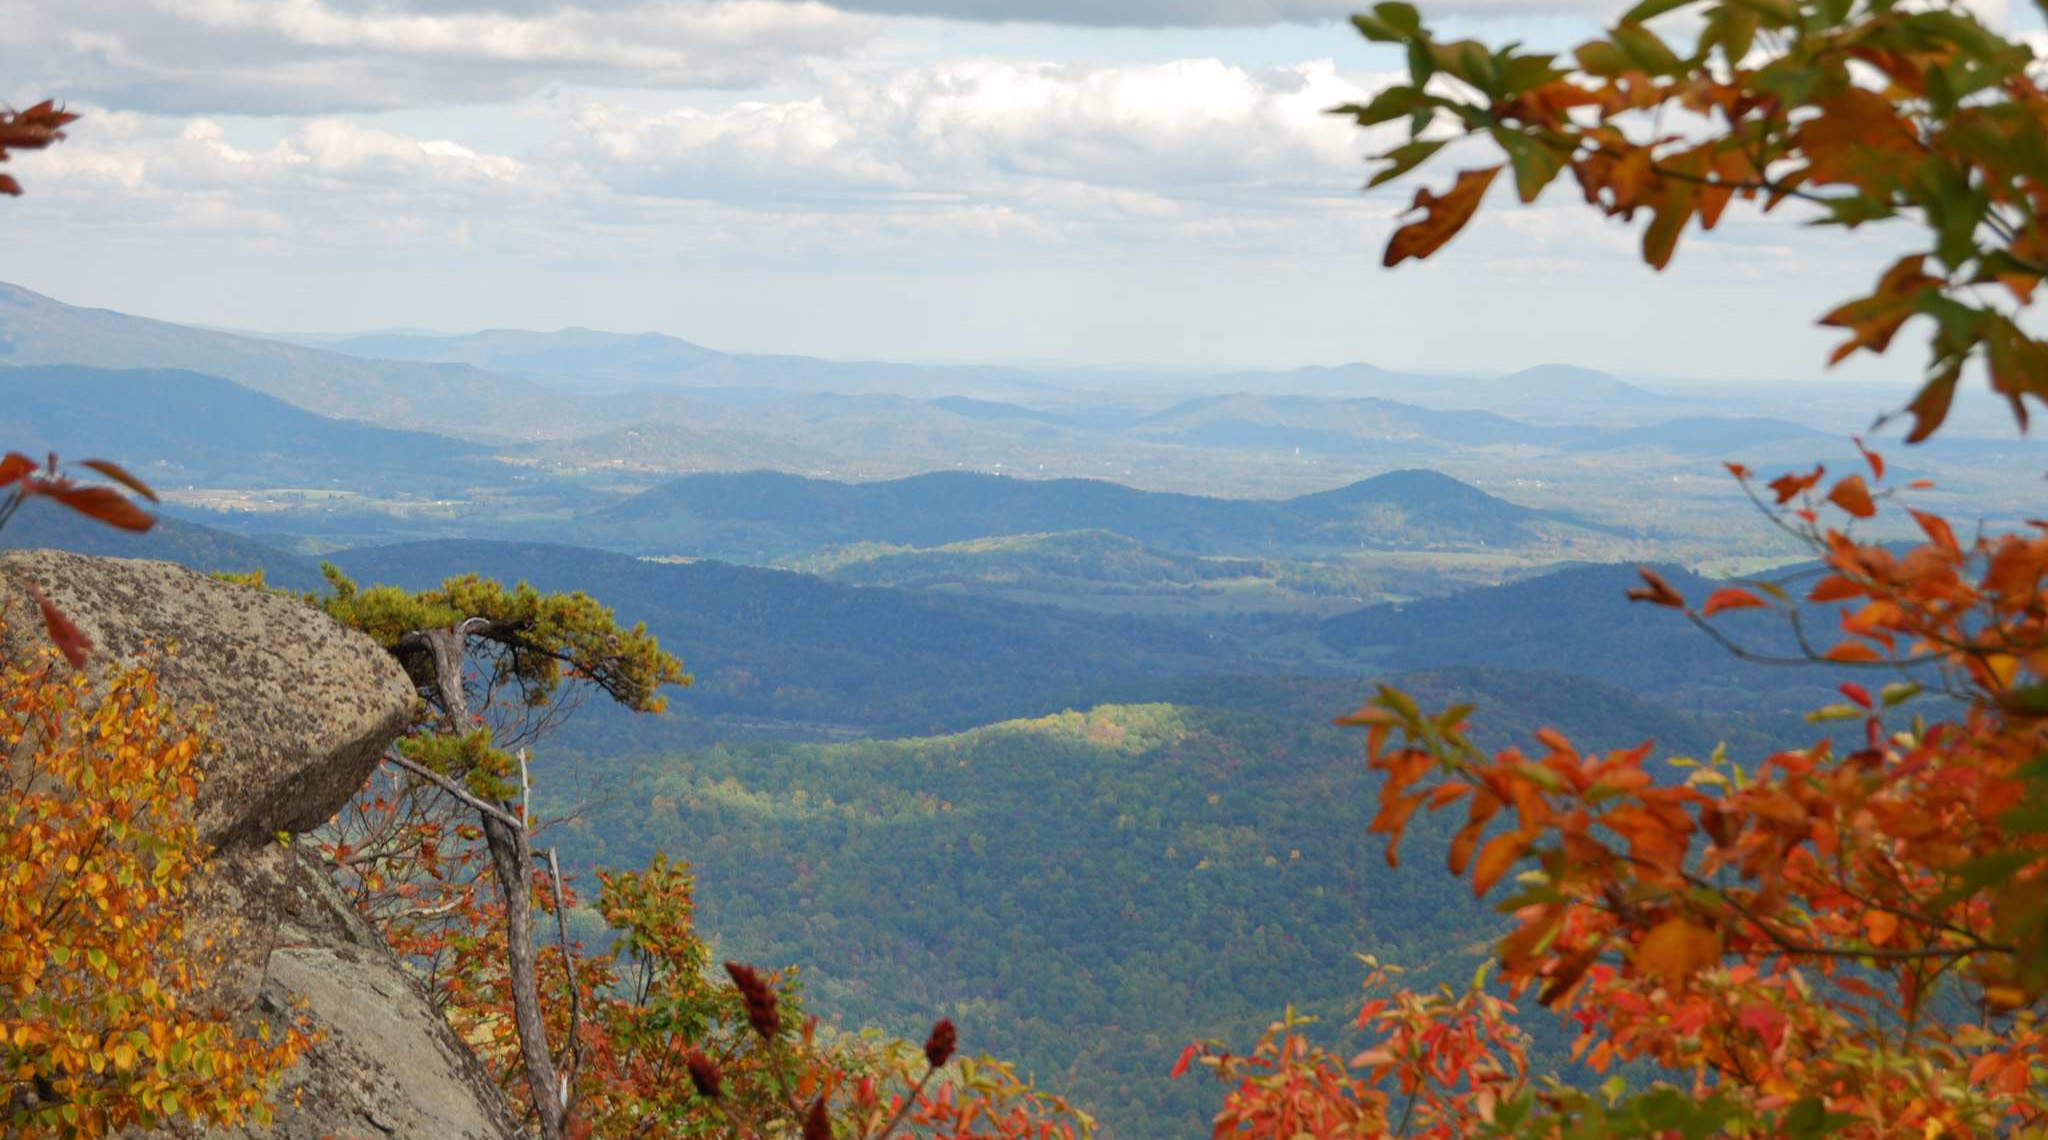
\includegraphics[width=\linewidth]{view}
%	\caption{Wide Picture}
%	\label{fig:view}
%\end{figure*}

%------------------------------------------------
\subsection{Procedimiento experimental}
%\label{subsec:procedimiento-experimental}
%------------------------------------------------

A continuación, será necesario redactar \textit{explícitamente} (itálicas \verb|\textit{}|) todo el procedimiento experimental seguido; si la naturaleza del artículo requiere dividir esta subsección, puede utilizarse el comando \verb|\subsubsection{}|.

Suele explicarse el diseño de muestreo (cantidad de muestras, cómo se obtuvieron, en qué condiciones), diseño experimental (controles, tratamientos, variables), análisis de datos (cómo se analizaron, procedimientos estadísticos), entre otra información relevante.
%------------------------------------------------
%%%%%%%%%%%%%%%%%%%%%%%%%%%%%%%%%%%%%%%%%%%%%%%%
\section{Resultados} % NOMBRE DE LA SECCIÓN
\label{sec:resultados} % ETIQUETA
%%%%%%%%%%%%%%%%%%%%%%%%%%%%%%%%%%%%%%%%%%%%%%%%

Los resultados deberán mostrar una secuencia lógica y deberán contener toda la información necesaria para su futura interpretación; si la naturaleza de los experimentos lo requiere, estos deben de presentarse en subsecciones. Con el objetivo de mostrar la información generada de una manera amigable y comprensible, se requiere utilizar tablas y figuras autoexplicativas. Es importante destacar que en esta sección no se describe por qué se obtuvieron estos resultados, ya que esto se realizará más adelante en la sección \ref{sec:discusion}.

A continuación, se mostrarán ejemplos de cómo insertar tablas y figuras, incluidas sus correspondientes descripciones; además, se explicará como agregar ecuaciones químicas. Por ejemplo, en la figura \ref{fig:xrd} se muestra un difractograma de rayos X (XRD) de nanopartículas de óxido de cobre (II) (NPs $CuO$) sintetizadas por el método de sol-gel.

\begin{figure}[ht!]
    \centering
    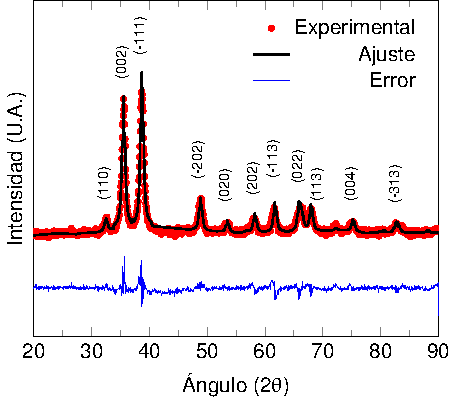
\includegraphics[width=\linewidth]{figuras/xrd.pdf}
    \caption{Difractograma de rayos X de NPs CuO; los planos cristalográficos característicos y que coinciden con la carta \textit{PDF Card No.: 01-089-5897 Quality: S} $Massarotti1998$.}
    \label{fig:xrd}
\end{figure}

El código para insertar la imagen puede encontrarse en el código fuente; la imagen anterior es un archivo \texttt{.pdf} (paquete \texttt{pdfpages}), sin embargo, es posible utilizar archivos \texttt{.png} y \texttt{.jpg}/\texttt{.jpeg}; incluso, es posible agregar archivos \texttt{.tif} (generalmente obtenidos en imagenes de SEM) directamente al código ya que el preámbulo contiene un código que permite su conversión a \texttt{.png}.

Definitivamente, el diseño de tablas es uno de los procesos más complejos en \LaTeX; con el objetivo de agilizar esto, se sugiere arreglar la información en una hoja de Microsoft Excel y utilizar la página \href{https://www.tablesgenerator.com/}{\textcolor{blue}{Tables Generator}} y seleccionar \textit{Escape special \TeX~symbols (\%, \&, \_, \#, \$)}, \textit{Smart output formatting} y en opciones extra \textit{Center table horizontally}. Además, en el archivo \texttt{0.0\_seccion.tex} en la carpeta \textit{secciones} de esta plantilla se encuentra el formato de tabla deseado. En caso de colocar una tabla que abarque ambas columnas de la página, se debe utilizar el ambiente \texttt{table*}.

Aunque existen otros paquetes con el mismo objetivo, el autor de esta plantilla sugiere el uso del paquete \texttt{mhchem}, cuya \href{https://mirrors.rit.edu/CTAN/macros/latex/contrib/mhchem/mhchem.pdf}{\textcolor{blue}{documentación}} puede encontrarse en la red, para el uso de redacción de compuestos y ecuaciones químicas. Este paquete requiere el uso del comando \verb|\ce{}|, el cual puede usarse directamente en párrafos, por ejemplo, para escribir $H2O$, $CH3CH2OH$, $CrO4^2-$, o bien arreglar reacciones químicas tal como en la ecuación \eqref{eq:rxn-1}.

\begin{equation}
    \label{eq:rxn-1}
    $C3H8(g) + 5 O2(g) -> 3 CO2(g) + 4 H2O(g)$
\end{equation}

\noindent Es de suma importancia leer la documentación para evitar caer en errores de uso de flechas, subíndices y coeficientes; el código utilizado para la redacción de la ecuación anterior es el siguiente:

\begin{verbatim}
    \begin{equation}
        \label{eq:rxn-1}
        \ce{C3H8(g) + 5O2(g) -> 3 CO2(g) 
            + 4H2O(g)}
    \end{equation}
\end{verbatim}
%-------------------------------------------------
%%%%%%%%%%%%%%%%%%%%%%%%%%%%%%%%%%%%%%%%%%%%%%%%
\section{Discusión de resultados} % NOMBRE DE LA SECCIÓN
%\label{sec:discusion} % ETIQUETA
%%%%%%%%%%%%%%%%%%%%%%%%%%%%%%%%%%%%%%%%%%%%%%%%

En la discusión de resultados se realiza un análisis profundo, objetivo y lógico de la información experimental presentada en la sección anterior; es de importancia comparar los resultados de este trabajo con investigaciones previas, por lo que en esta sección deberán observarse citas a diversas referencias de fuentes confiables. Para cualquier explicación teórica, deberá utilizarse una fuente para sustentar este dicho.

Con respecto a los títulos de las figuras y tablas, estos deben sintetizar la información más relevante y necesaria para comprender el gráfico o datos presentados; por ejemplo, es importante mencionar la cantidad de muestras analizadas, las condiciones de temperatura, presión, tiempo, etc., el equipo utilizado para la medición, entre otros puntos. En tablas, la descripción siempre se encuentra en la parte superior, mientras que en las figuras se coloca en la parte inferior de estas.


%\begin{table}[hbt]
%	\caption{Table of Grades}
%	\centering
%	\begin{tabular}{llr}
%		\toprule
%		\multicolumn{2}{c}{Name} \\
%		\cmidrule(r){1-2}
%		First name & Last Name & Grade \\
%		\midrule
%		John & Doe & $7.5$ \\
%		Richard & Miles & $2$ \\
%		\bottomrule
%	\end{tabular}
%	\label{tab:label}
%\end{table}



\begin{table*}[ht!]
\centering
\caption{Concentraciones establecidas de nanopartículas de CuO y Pb en las muestras de agua destilada a 25 mL. Las muestras M-A y M-B no pudieron ser cuantificadas ya que la concentración de plomo después del tratamiento se encontró debajo del límite de detección (DLD), lo cual podría indicar una alta capacidad de adsorción de plomo.\\}

    \begin{tabular}{c|crrrr|r}
    
        \toprule
        \textbf{ID} & \textbf{NPs (mg)} & \multicolumn{1}{c}{\textbf{$C_0$ Pb (mg L$^{-1}$)}} & \multicolumn{1}{c}{\textbf{$C_f$ Pb (mg L$^{-1}$)}} & \multicolumn{1}{c}{\textbf{\% Adsorción}} & \multicolumn{1}{c}{\textbf{$C_e$ (mg L$^{-1}$)}} & \multicolumn{1}{c}{\textbf{$q_e$ (mg g$^{-1}$)}} \\
        \midrule
        M-A         & 18                & 0.00                                                     & DLD                                                      & -                                        & -                                                & -                                                \\
        M-B         & 20                & 5.00                                                     & DLD                                                      & -                                        & -                                                & -                                                \\
        M-C         & 18                & 10.00                                                    & 7.21                                                     & 27.87                                    & 7.2129                                           & 103.5179                                         \\
        M-D         & 19                & 20.00                                                    & 5.78                                                     & 71.10                                    & 5.7796                                           & 18.7111                                          \\
        M-E         & 19                & 40.00                                                    & 18.67                                                    & 53.32                                    & 18.6719                                          & 28.0633                                          \\
        M-F         & 20                & 80.00                                                    & 51.01                                                    & 36.24                                    & 51.0111                                          & 36.2361                                          \\
        M-G         & 19                & 100.00                                                   & 51.95                                                    & 48.05                                    & 51.9451                                          & 63.2301                                          \\
        M-H         & 20                & 120.00                                                   & 67.45                                                    & 43.79                                    & 67.4486                                          & 65.6892                                         \\
        \bottomrule
    
    \end{tabular}

\label{tab:adsorcion}
\end{table*}

%------------------------------------------------
%%%%%%%%%%%%%%%%%%%%%%%%%%%%%%%%%%%%%%%%%%%%%%%%
\section{Conclusiones} % NOMBRE DE LA SECCIÓN
\label{sec:conclusiones} % ETIQUETA
%%%%%%%%%%%%%%%%%%%%%%%%%%%%%%%%%%%%%%%%%%%%%%%%

Las conclusiones deben ser concisas y mostrar en forma de resumen los resultados más relevantes obtenidos, específicamente, agregando valores numéricos y frases que describan la diferencia observada en los experimentos de este trabajo en comparación con otros proyectos. Se sugiere también agregar al menos dos aplicaciones actuales o potenciales para el material o método desarrollado y su importancia en el mercado.

Aunque generalmente las conclusiones se redactan en forma de párrafo, algunos autores deciden presentar sus resultados en viñetas o en lista numerada:\vspace{1ex}

\begin{itemize}
    \item En el código se fuente de esta plantilla se muestra cómo agregar viñetas al documento
    \item Es posible también agregar sub-viñetas:
    \begin{itemize}
        \item por ejemplo, esta línea de texto
    \end{itemize}
\end{itemize}

\vspace{1ex} \noindent Sin embargo:\vspace{1ex}

\begin{enumerate}
    \item Las conclusiones pueden también enumerarse tal como se mencionó previamente
    \item No necesariamente esto represente la importancia de los resultados, sino el orden en que fueron presentados
\end{enumerate}

\vspace{1ex} Esta plantilla tiene diversos campos cargados con el paquete \texttt{hyperref} en el archivo \texttt{preambulo.sty}, el cual contiene todos los paquetes requeridos para la compilación de este documento, donde se deben colocar el título interno del archivo \texttt{.pdf} generado, el o los autores, el asunto y palabras claves; uno o más de estos campos pueden dejarse vacíos. Si se desea agregar la fecha actual, se puede utilizar el comando \verb|\today|. Al compilar se generará un error si en los campos se utilizan tildes y otros caracteres no nativos del inglés. \cite{Figueredo:2009dg}
%----------------------------------------------

\phantomsection
\section*{Agradecimientos} % The \section*{} command stops section numbering

\addcontentsline{toc}{section}{Acknowledgments} % Adds this section to the table of contents

So long and thanks for all the fish \cite{Figueredo:2009dg, Smith:2012qr}.

%----------------------------------------------------------------------------------------
%	REFERENCE LIST
%----------------------------------------------------------------------------------------

\phantomsection
\bibliographystyle{unsrt}
\bibliography{sample.bib}

%----------------------------------------------------------------------------------------

\end{document}















